\documentclass[10pt]{article}
\newcommand{\HRule}{\rule{\linewidth}{0.5mm}}
\parindent 0pt
\parskip 10pt
\usepackage{anysize}
\usepackage{graphicx}
\usepackage{epsfig}
\usepackage{float}
%\usepackage{cite}
\usepackage{natbib}
\usepackage{setspace}
\marginsize{3.5cm}{3.5cm}{1cm}{1cm}
\onehalfspacing
\usepackage{caption}
\usepackage{subcaption}
\usepackage{amsmath,hyperref}

\usepackage{xcolor}
\hypersetup{
    colorlinks,
    linkcolor={red!50!black},
    citecolor={blue!50!black},
    urlcolor={blue!80!black}
}

%\textwidth 15cm
%\textheight 24cm
%\onehalfspacing
\begin{document}

\title{Bike Forecast}

\author{David Starkey}

\maketitle





\section{Introduction and Data Ingestion}
This project provides the details of bike hires in Montreal Canada dating from 2014 up to August 2017. The goal is to use statistical models to forecast the expected daily number of bike hires between two stations ( and ) for one weeks worth of hires between 4th September 2017 and 11th September 2017. Each bike hire records the date, departure station and arrival station. This data is contained within several csv files which collectively total 15.3 million entries.

This summary is presented as follows. Section \ref{sec_ingest} details the data ingestion process. Section \ref{sec_exp} presents the findings of the initial exploratory data analysis and includes several figures that motivate the choice of fitted-model in the subsequent sections. The mathematical theory is presented in Section \ref{sec_model} and the results of the model fitting are provided in Section \ref{sec_results}.


\section{Data Ingestion}
\label{sec_ingest}
The script \verb|prep_data.py| loads all the information from all the Excel csv files into a python Pandas data frame. Pandas data frames are extremely useful objects that I use to convert the time in date format xx/xx/xxxx to an integer number of days relative to a reference point (chosen as 1st January 2014). Many of the commands in \verb|prep_data.py| are remenants of earlier data analysis but the key ouputs of this script are the \verb|'labels_station.csv'| and \verb|'labels_info.csv'| files. These contain the time series of the entire combined sample (in number of trips as a function of day), and the time series restricted to trips between stations 6184 to 6015. The time series fitting is performed in the script \verb|'myfitrw_092018.py'|. The output forecasts are written to files \verb|'predictions_arma_station.txt'| for the specific station and \verb|'predictions_drw_fullsample.txt'| for the fit to the global sample.


\section{Exploratory Data Analysis}
\label{sec_exp}

\subsection{Time Series}
Before deciding how best to model the forecasting problem, a universally sound first step is to visualise the data. I use Pythons matplotlib module to plot the number of bike hires as a time series, concatenating all four years of observations together. Figure \ref{fig_ts} presents some very important information on the Time Series

\begin{itemize}
\item The time series is periodic. It exhibits a similar annual pattern with bike hires becoming more popular in the summer months.

\item The amplitude of the variations appears to be increasing over time (smooth red line Figure \ref{fig_ts}). This suggests bike hires are increasing in popularity.
\end{itemize}




\begin{figure}
\begin{center}
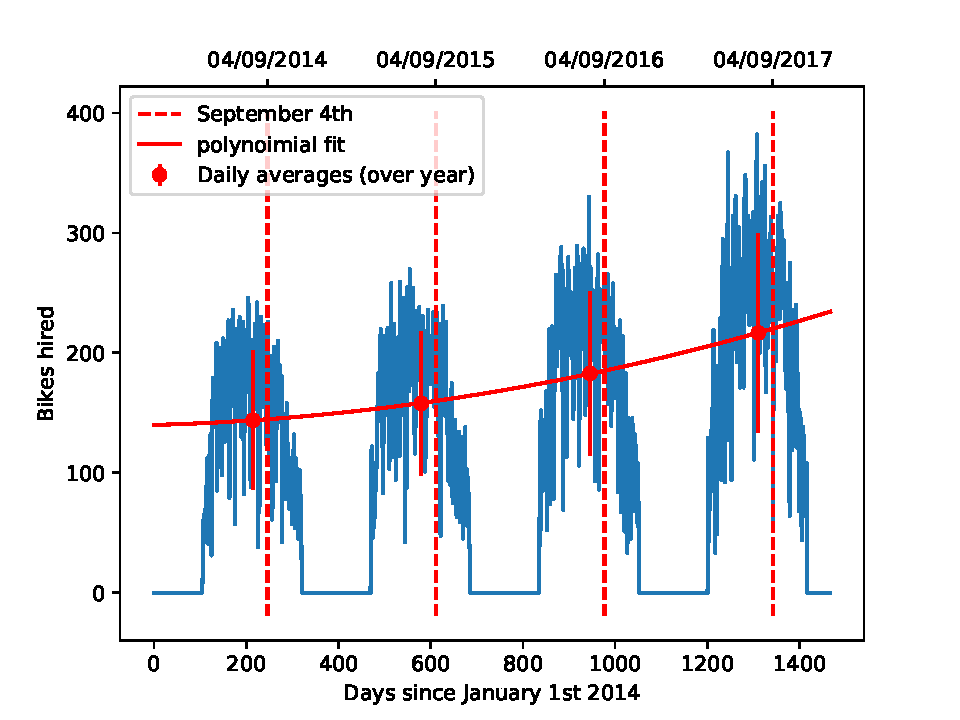
\includegraphics[scale=1.0,angle=0,trim=0cm 0cm 0cm 0cm]{ts_plot.pdf}
\caption{Time series of bike hires. Y axis plots the number of bikes hired per day as a function of day number (days are measured relative to 1st January 2014). The vertical red dashed lines show 4th September of each year (the start of the forecast week) and the smooth vertical polynomial fit shows how the average daily number of bike hires increases over the four years of data.}
\label{fig_ts}
\end{center}
\end{figure}
\begin{figure}
\begin{center}
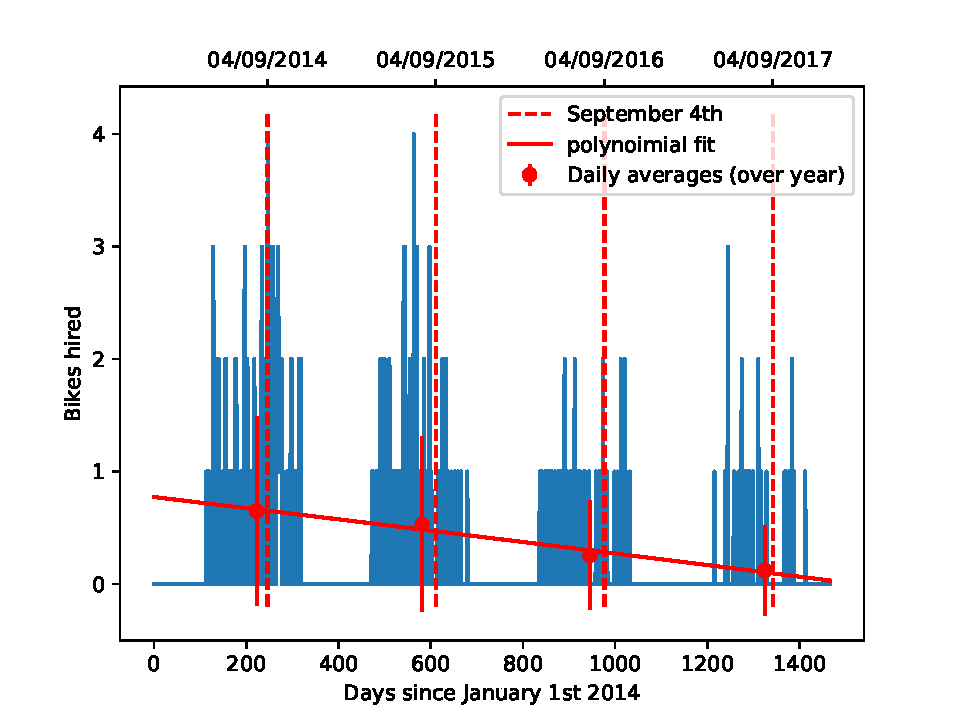
\includegraphics[scale=1.0,angle=0,trim=0cm 0cm 0cm 0cm]{ts_plot_station.pdf}
\caption{Same as Figure \ref{fig_ts} but restricting the time series only to bike hires departing at station 6184 and ending at station 6015.}
\label{fig_ts_station}
\end{center}
\end{figure}




While Figure \ref{fig_ts} provides useful information on the periodicity of the time series, this information is much clearer to see when presented as a power spectrum. The power spectrum as a function of frequency $P(f)$ can be computed from the Fourier transform of time-series data $F(f)$ where

\begin{equation}
\label{eq_ft}
F(f) = \int_{-\infty}^{\infty} f(t) e^{-2\pi f t} dt,
\end{equation}
\noindent and $P(f)$ is then

\begin{equation}
\label{eq_ps}
P(f) = F^*(f) F(f),
\end{equation}

\noindent where $*$ denotes complex conjugation. Qualitatively, the power spectrum $P(f)$ tells us if there are strong periodic features in our data set. Figure \ref{fig_ps} demonstrates that the bike hires in this data set go through seasonal and weekly cycles of popularity, likely due to the seasonal weather / holiday season and weekend trend increases.





\begin{figure}
\begin{center}
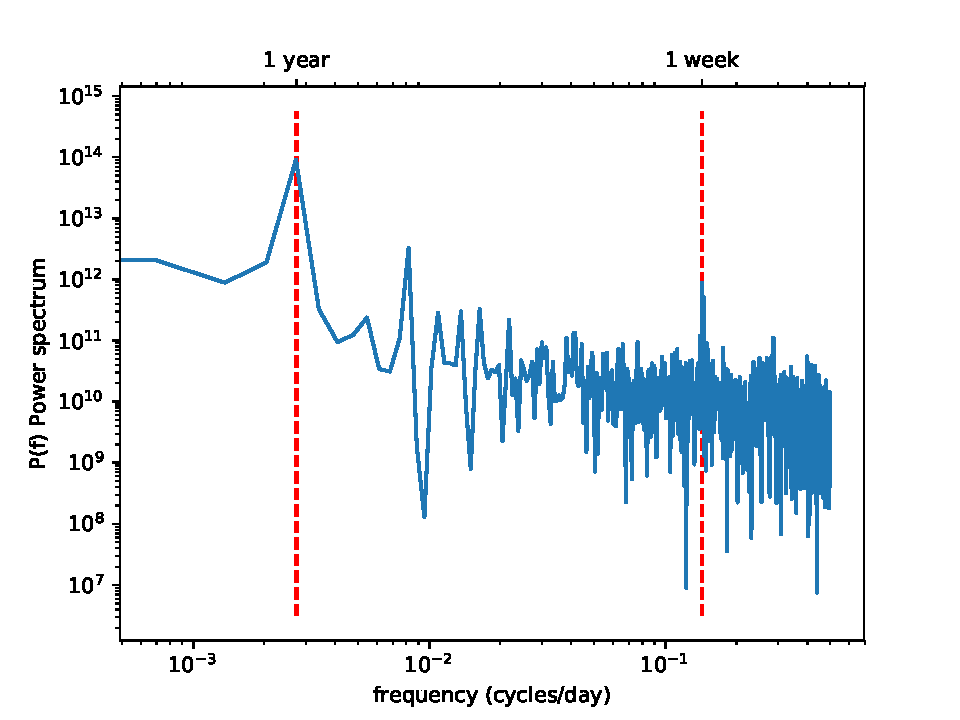
\includegraphics[scale=1.0,angle=0,trim=0cm 0cm 0cm 0cm]{ps_plot.pdf}
\caption{Power spectrum $P(f)$ versus frequency of the time series data presented in Figure \ref{fig_ts}. The peaks at one year and one week timescales (red dashed lines) show that bike hire goes through seasonal and weekly cycles of popularity.}
\label{fig_ps}
\end{center}
\end{figure}






\section{Model fitting (Modified random walk and ARMA models)}
\label{sec_model}


Now that the periodicity of the bike hires is better understood, I will fit a model to the global sample to forecast the bike hires for the week beginning 4th September 2017. The model I use here is a variant on the Random walk approach used in forecasting time series data for flickering galaxies. The model not only forecasts but interpolates between data gaps. The random walk model exhibits a logarithmic power spectrum slope of -2 similar to the power spectrum of the bike data here in Figure \ref{eq_ps}. We also note from Figure \ref{fig_ps} significant power at frequencies of 1 year and 1 week respectively indicating some additional periodicity in excess of a damped random walk model.

The full fitted model is therefore given by

\begin{equation}
\label{eq_rwmod}
f(t_i) = \sum_k S_K \sin \left( \omega_k t_i \right) + C_k \cos \left( \omega_k t_i \right)
\end{equation}

Here the sine and cosine amplitudes at each frequency $S_k$ and $C_k$ are regularized by the random walk prior to prevent the high frequencies from over-fitting the data. As with many model fitting problems, the optimum amplitudes $S_k$ and $C_k$ are found by minimizing a cost function $E$, where $E$ is determined not only by how well the model fits the data ($\chi^2$), but whether the fit obeys the priors on the model parameters that regularize the high frequencies against over-fitting. The full cost function therefore takes the form 
\begin{equation}
\label{eq_cost}
\chi^2 = \sum_i \left( D(t_i)-f(t_i) \right)^2 + \sum_k \frac{ S_k^2 + C_k^2 }{\sigma_k^2} ,
\end{equation}
\noindent where $D$ is the time series data and $f(t)$ is the model given in Equation \ref{eq_rwmod}. The prior distribution with width $\sigma_k$ at each frequency $\omega_k$ is given by

\begin{equation}
\label{eq_prior}
\sigma_k^2 = P_0 \Delta \omega_k \left( \frac{\omega_k}{\omega_0}\right)^{-2}.
\end{equation}



The parameter vector $\mathbf{\theta}$ is explicitly given by

\begin{equation}
\mathbf{\theta} = \theta \left(S_{k=1},C_{k=1} ...S_{k=N_k},C_{k=N_k} \right),
\end{equation}


In general, one can optimize the model parameters by differentiating $\chi^2$ with respect to each parameter and forming a `Hessian' Matrix $\underline{\underline{\mathbf{H}}}$ \footnote{Double underline here means a $N$ by $N$ matrix where $N$ is just the number of model parameters} out of the resulting system of equations such that.

\begin{equation}
\label{eq_hes}
\underline{\underline{\mathbf{H}}} \mathbf{\theta} = \mathbf{c(Y)},
\end{equation}
\noindent where $c(Y)$ is a constant vector dependent only on the observations $Y$, but not the parameters $\mathbf{\theta}$. The parameter vectors are then given by inverting this matrix and rearranging to form 
\begin{equation}
\label{eq_hespars}
\mathbf{\theta} = \underline{\underline{\mathbf{H}}}^{-1} \mathbf{c(Y)}.
\end{equation}


This optimization function is defined in a python script \verb|myfitrw_092018| from my own library and is included in this bundle. For smaller sample sizes, I use an Auto Regressive Moving Average (ARMA) code to model the time series. Since we are interested in forecasting trips between station 6184 and 6085, we will be restricting our sample to small numbers and will require a model such as ARMA to perform the fit. ARMA also models are ideal for forecasting time series data and in general take the form

\begin{equation}
\label{eq_arma}
Y(t) = C + G(0,\sigma^2) + \sum_{i=1}^{p} A_i Y(t_{i-1}) + \sum_{i=1}^{q} B_i G(0,\sigma^2)
\end{equation}


\noindent where $C$ is the background level of the time series, $G(0,\sigma^2)$ indicates a draw from a Gaussian distribution with mean $0$ and variance $\sigma^2$. Although the model is different from the RW-mod model shown in Figure \ref{eq_rwmod}, the optimization technique of minimizing the cost function is the same, although cannot be solved analytically in the case of th ARMA model \footnote{Various texts exist for numerical optimization of ARMA  parameters (see for example \href{ http://www.phdeconomics.sssup.it/documents/Lesson12.pdf}{\textcolor{blue}{http://www.phdeconomics.sssup.it/documents/Lesson12.pdf}}).}.









\section{Results}
\label{sec_results}
The RW-mod model is trained on the history of bike hire time series observations (Figure \ref{fig_ts}) up to the 31st August 2017. The remaining entries in the csv file serve only as a bench mark test data set to test the models's accuracy. In Figures \ref{fig_drw_total} and \ref{fig_drw_zoom} , I first use the entire of the 2017 entries as the test data set to illustrate the predictive power of the DRW-mod model (in other words the model sees no data from 2017). It has been noted from past experience that RW-mod models perform poorly when fitted to data with low numbers of sample. One issue here is that there are very few trips exclusively between these stations on which to base a forecast (only 340 in fact). I instead fit the ARMA model to the reduced data set of trips between just stations 6184 and 6085. The result are shown in Figures \ref{fig_arma_station_total} and \ref{fig_arma_station_zoom}. We see here that although large uncertainty envelopes present themselves, the model performs a fair forecast of trips between the two stations. All results are consistent with zero to within the 1-$\sigma$ uncertainties (shaded red regions) and there were indeed zero trips between the selected stations in the week beginning 4th September 2018, proving the forecast correct. The resulting forecasts are outputed to the file \verb|predictions_drw_fullsample.txt| and for the full sample (using the RW-mod analysis) in \verb|predictions_arma_station.txt|. 




\begin{figure}
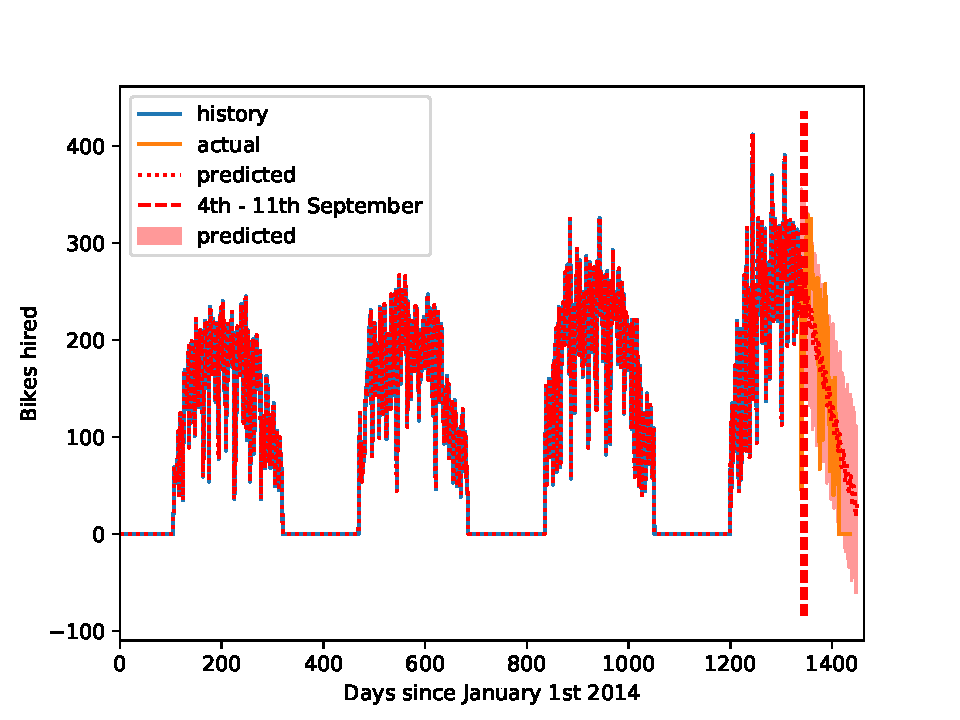
\includegraphics[scale=1.0,angle=0,trim=0cm 0cm 0cm 0cm]{drw_total_ts.pdf}
\caption{As with Figure \ref{fig_ts} but the red lines now show the RW-mod forecast beyond the final training data point (31st August 2017). Dashed red lines enclose the requested forecast period (4th - 11th September). Red shaded regions show the uncertainty envelopes.}
\label{fig_drw_total}
\end{figure}

\begin{figure}
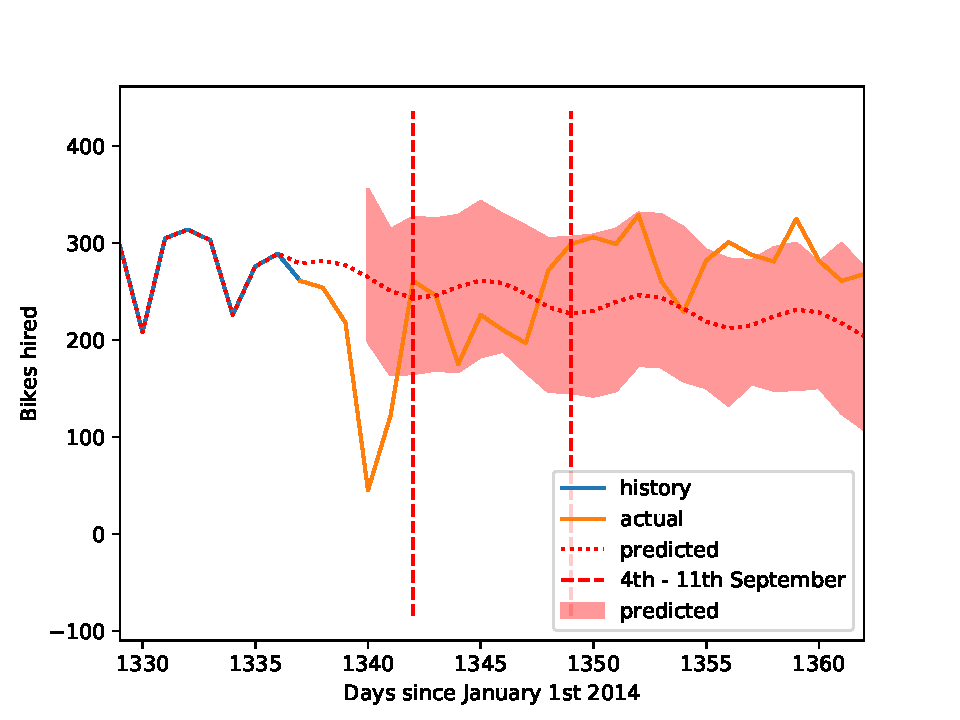
\includegraphics[scale=1.0,angle=0,trim=0cm 0cm 0cm 0cm]{drw_zoom_ts.pdf}
\caption{As with Figure \ref{fig_drw_total} but showing a zoom in of the requested forecast week (4th - 11th September).}
\label{fig_drw_zoom}
\end{figure}





\begin{figure}
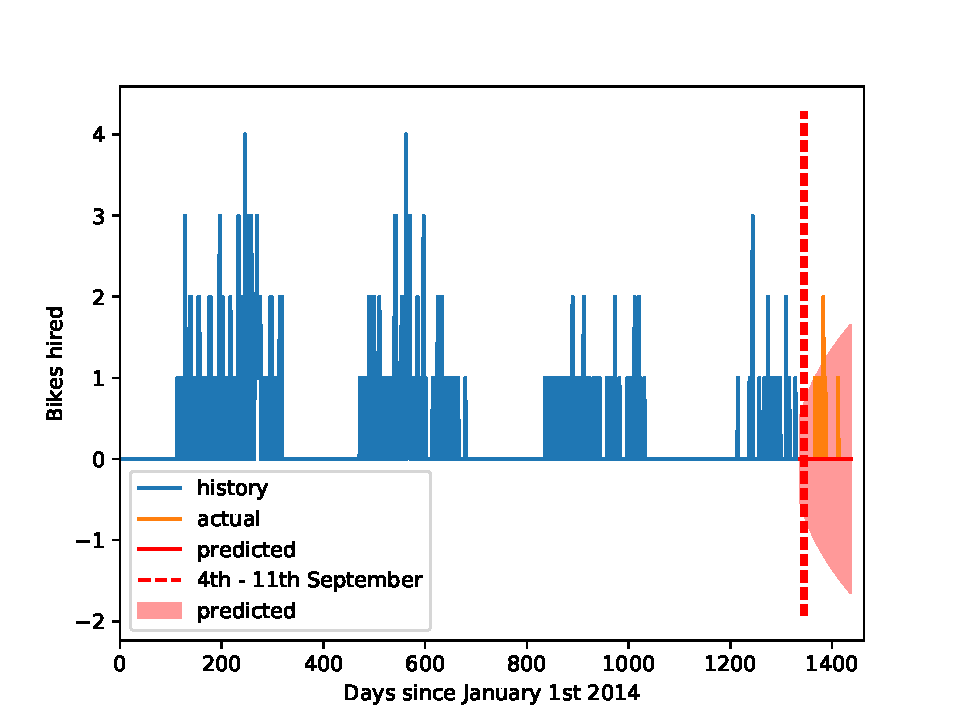
\includegraphics[scale=1.0,angle=0,trim=0cm 0cm 0cm 0cm]{arma_specstat_total.pdf}
\caption{As with Figure \ref{fig_drw_total} but showing only the forecasts between station 6184 6085.}
\label{fig_arma_station_total}
\end{figure}

\begin{figure}
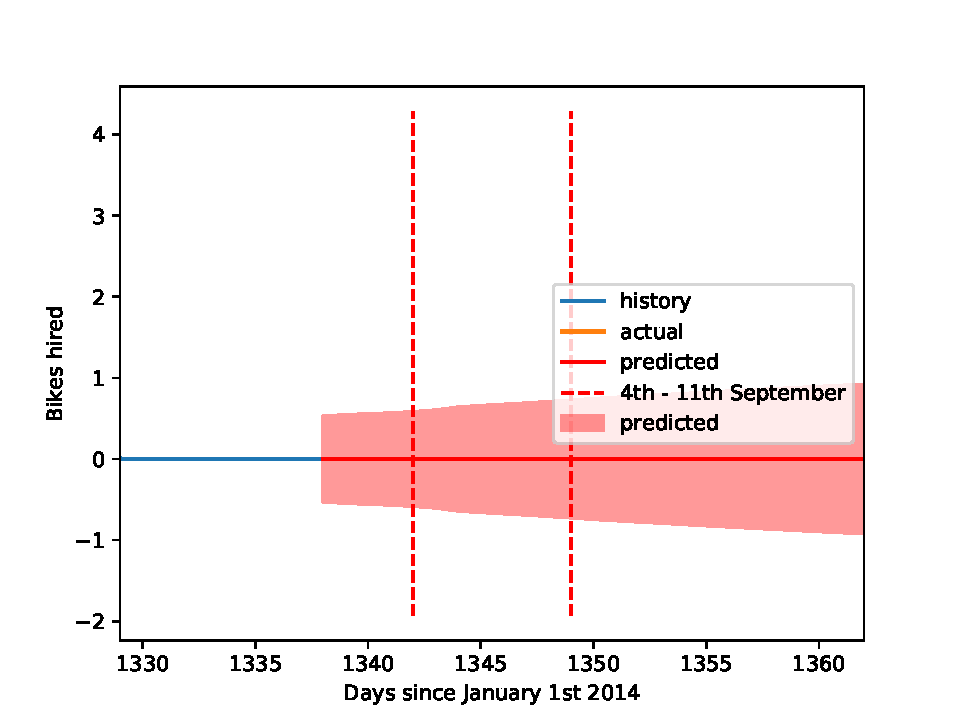
\includegraphics[scale=1.0,angle=0,trim=0cm 0cm 0cm 0cm]{arma_specstat_zoom.pdf}
\caption{As with Figure \ref{fig_arma_station_total} but showing a zoom in of the requested forecast week (4th - 11th September).}
\label{fig_arma_station_zoom}
\end{figure}






\section{Conclusions}
I have used various python modules including Pandas, Numpy, Csv, Keras and Matplotlib to ingest several million entries of bike hires between various stations in Montreal. I have visualised these data to identify periodic trends affecting the frequency of hires using a power spectrum analysis. I then forecast the expected frequency of hires (trips per day) for 1 week starting 4th September 2017 to both the global sample and specifically between Stations 6184 and 6085.

The RW-mod model n this forecast fits a Fourier tim series to the bike hire data with higher frequency coefficients regularized by a random walk prior to prevent over fitting. I allow additional un-regularized time-series components with frequencies of 1 year and 1 week respectively to give the model flexibility to fit the observed periodic features found in Figure \ref{fig_ps}. The predictions for the requested week forecast can be found in \verb|predictions_arma_station.txt| and for the full sample in \verb|predictions_drw_fullsample.txt|

ARMA models trialled in the appendix are also ideal for time series analysis but a potential draw back of the model is the need to specify in advance the number of autoregressive coefficients (the $p$ number of previous time series points to consider) and the number of moving average $q$ coefficients. Including too few of these can restrict the model and prevent it from fitting high frequency features or long term behaviour. Fitting too many of these can lead to over-fitting problems. A good check of the appropriate number of parameters to include in these models would be some form of Bayesian model regularisation check like the Bayesian Information Criterion (BIC). This includes a penalty into the cost function for models with large number of parameters and introduces a trade-off between a well fitting model and a reasonably small number of parameters. Such a check could form the basis of future investigations.

Thanks you for taking the time to review this analysis. 









\end{document}